
% Un anexo (o apéndice) es una sección adicional al final de un documento que proporciona información complementaria que no es esencial para el cuerpo principal del texto, pero que puede ser útil para el lector. Los anexos pueden incluir:

% - Datos adicionales o tablas extensas
% - Gráficos o diagramas detallados
% - Cuestionarios o formularios utilizados en la investigación
% - Códigos de programación
% - Documentación técnica
% - Resultados de pruebas o experimentos

\chapter{Anexo A}
\section{Cuestionario de evaluación de ergonomía}
lorem ipsum

\section{Resultados de pruebas de resistencia de ergonomía}
\begin{figure}[H]
    \centering
    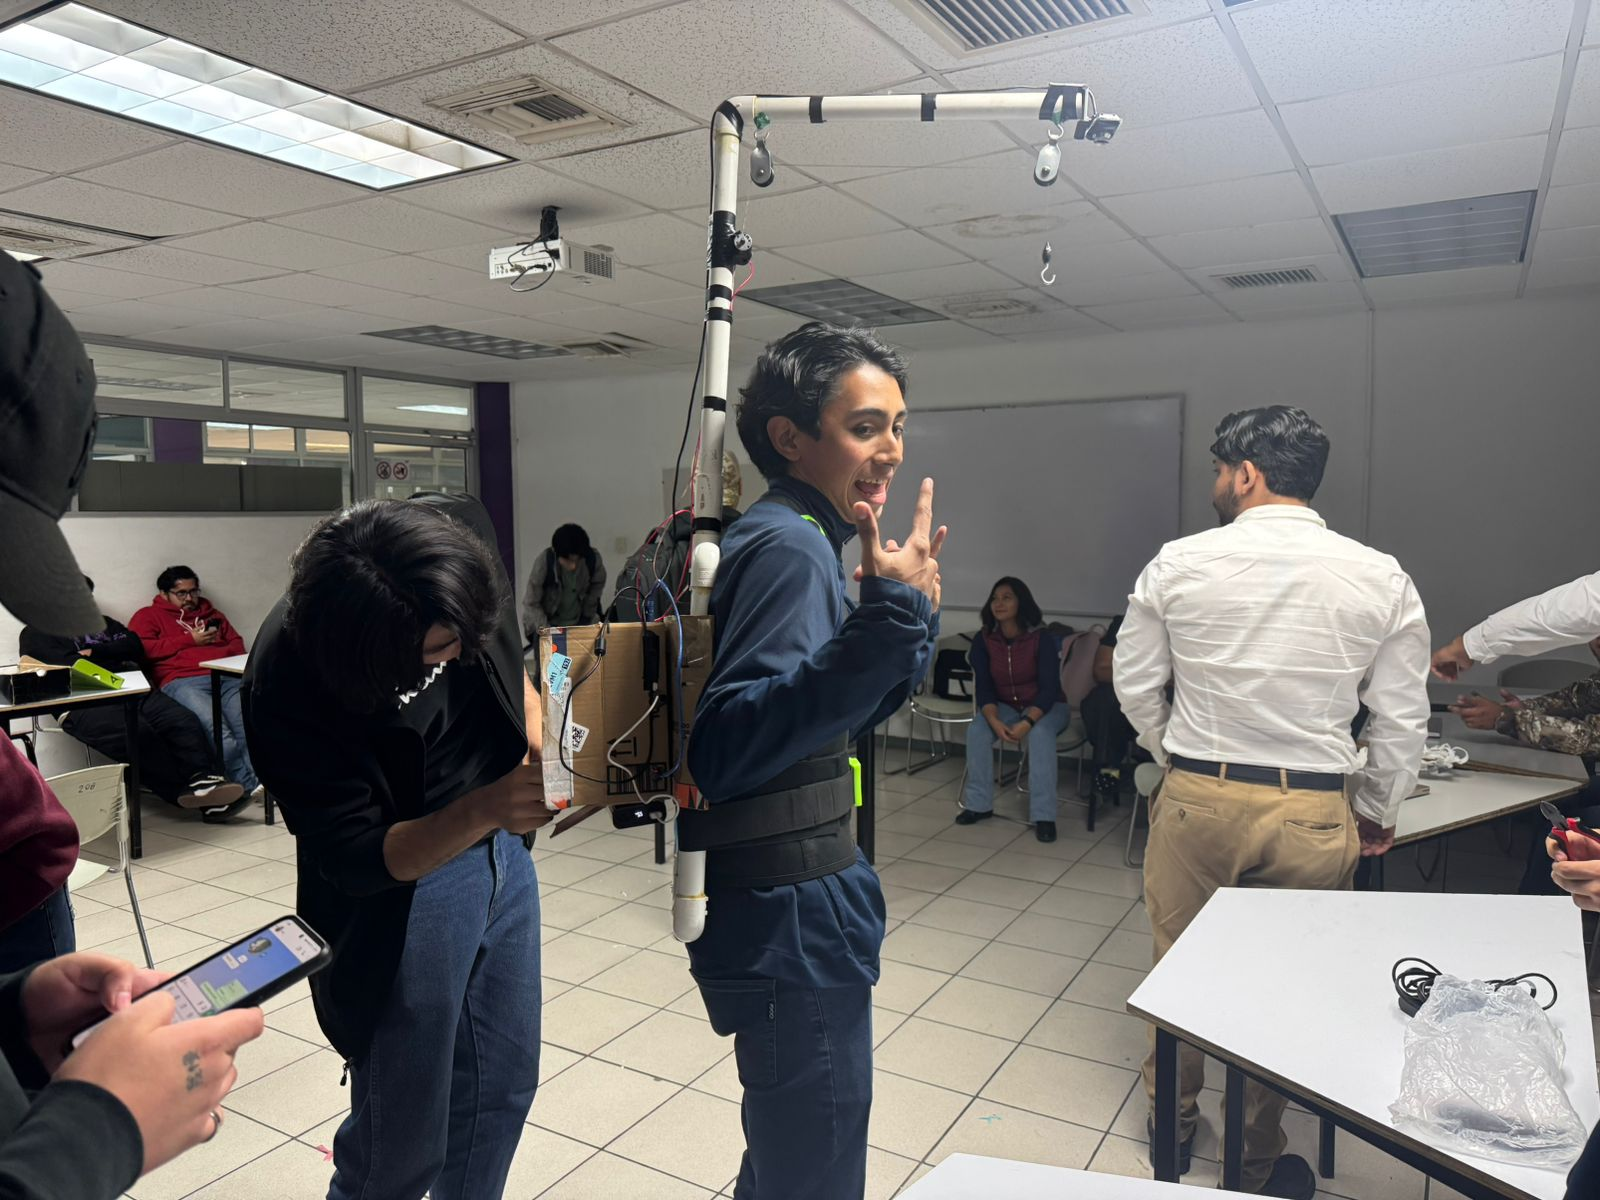
\includegraphics[width=1\textwidth]{img/PruebaErgonomica1.png}
    \caption{Resultados de pruebas de ergonomía}
    \label{fig:ergo-test1}
\end{figure}

\begin{figure}[H]
    \centering
    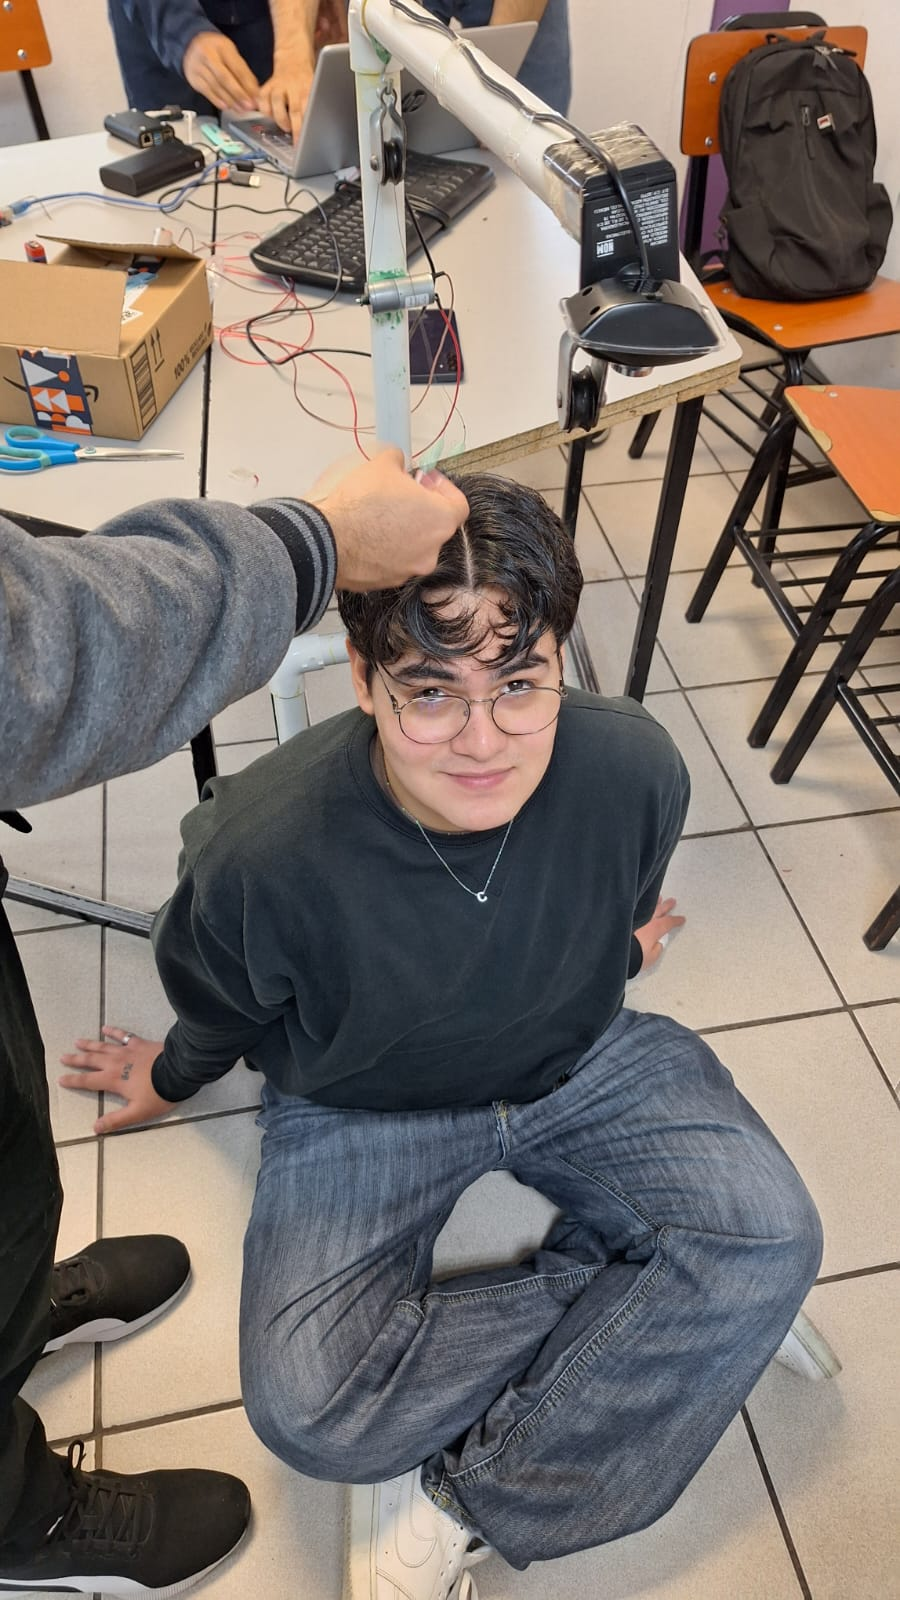
\includegraphics[width=1\textwidth, height=.9\textheight]{img/PruebaErgonomica2.png}
    \caption{Resultados de pruebas de ergonomía}
    \label{fig:ergo-test2}
\end{figure}

\begin{figure}[H]
    \centering
    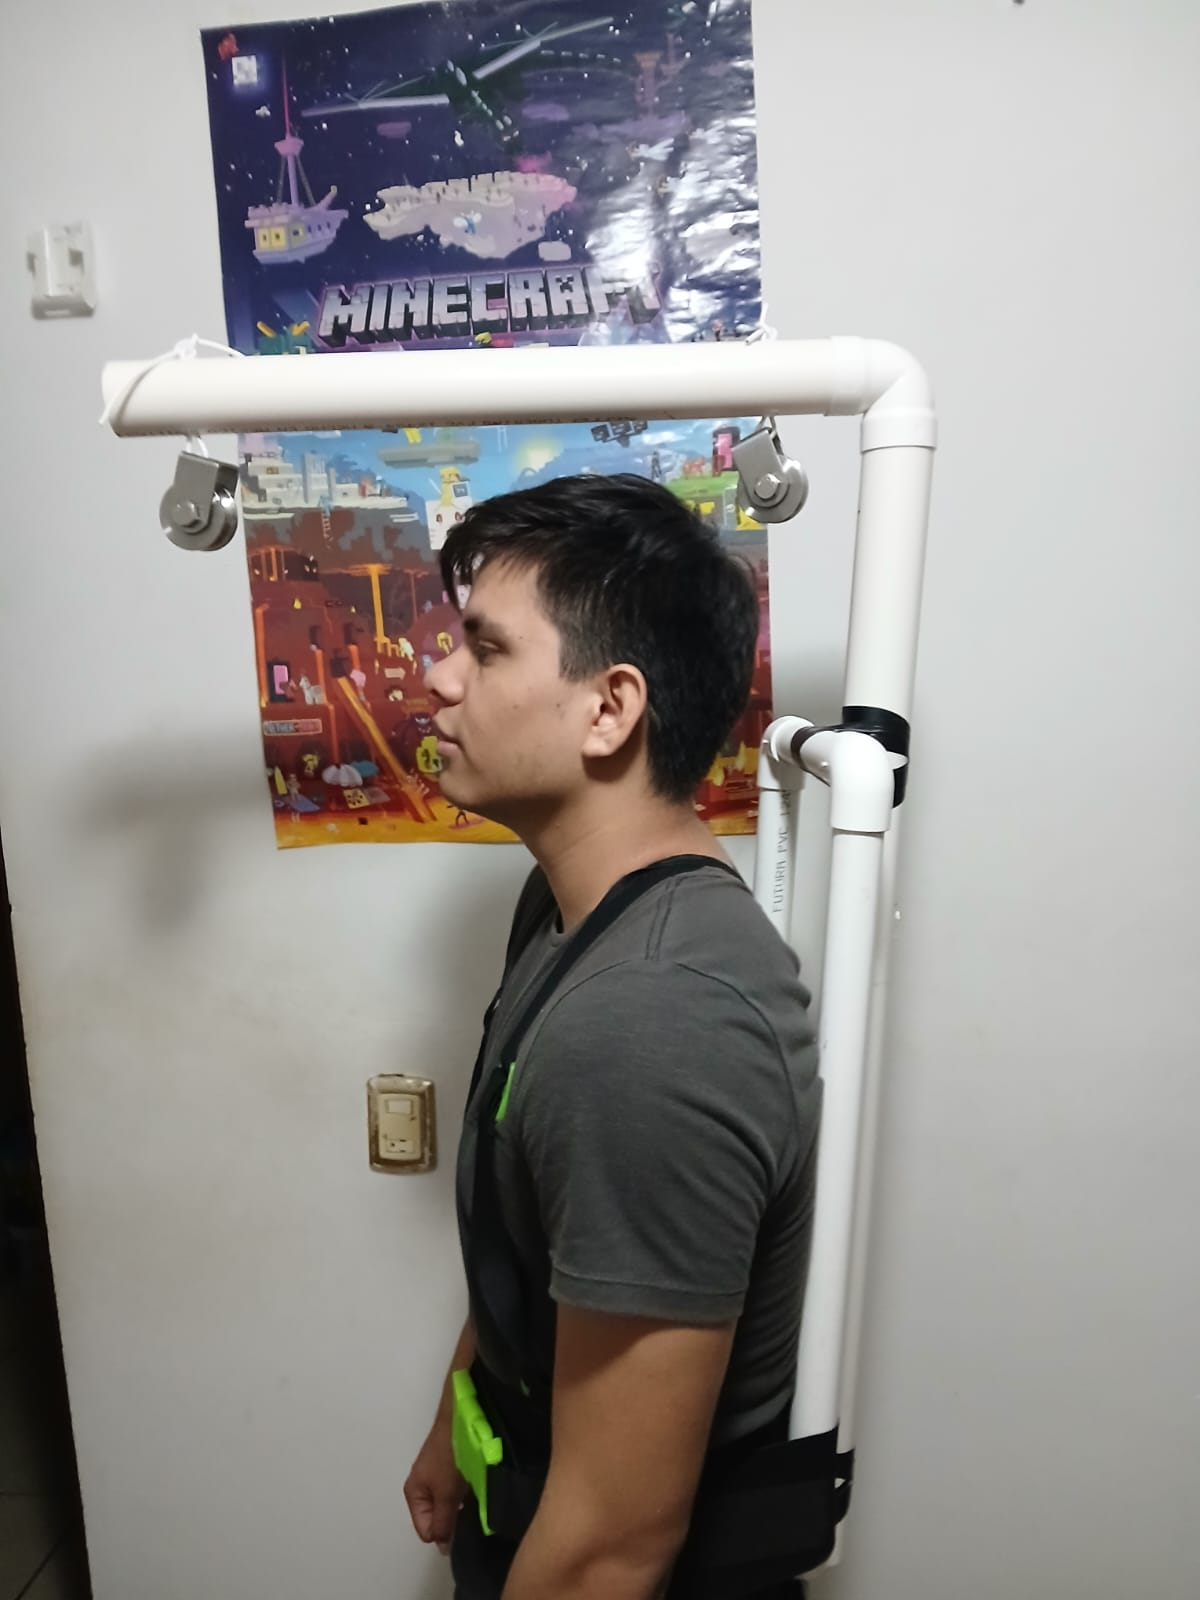
\includegraphics[width=1\textwidth, height=.9\textheight]{img/PruebaErgonomica3.png}
    \caption{Resultados de pruebas de ergonomía}
    \label{fig:ergo-test3}
\end{figure}

\begin{figure}[H]
    \centering
    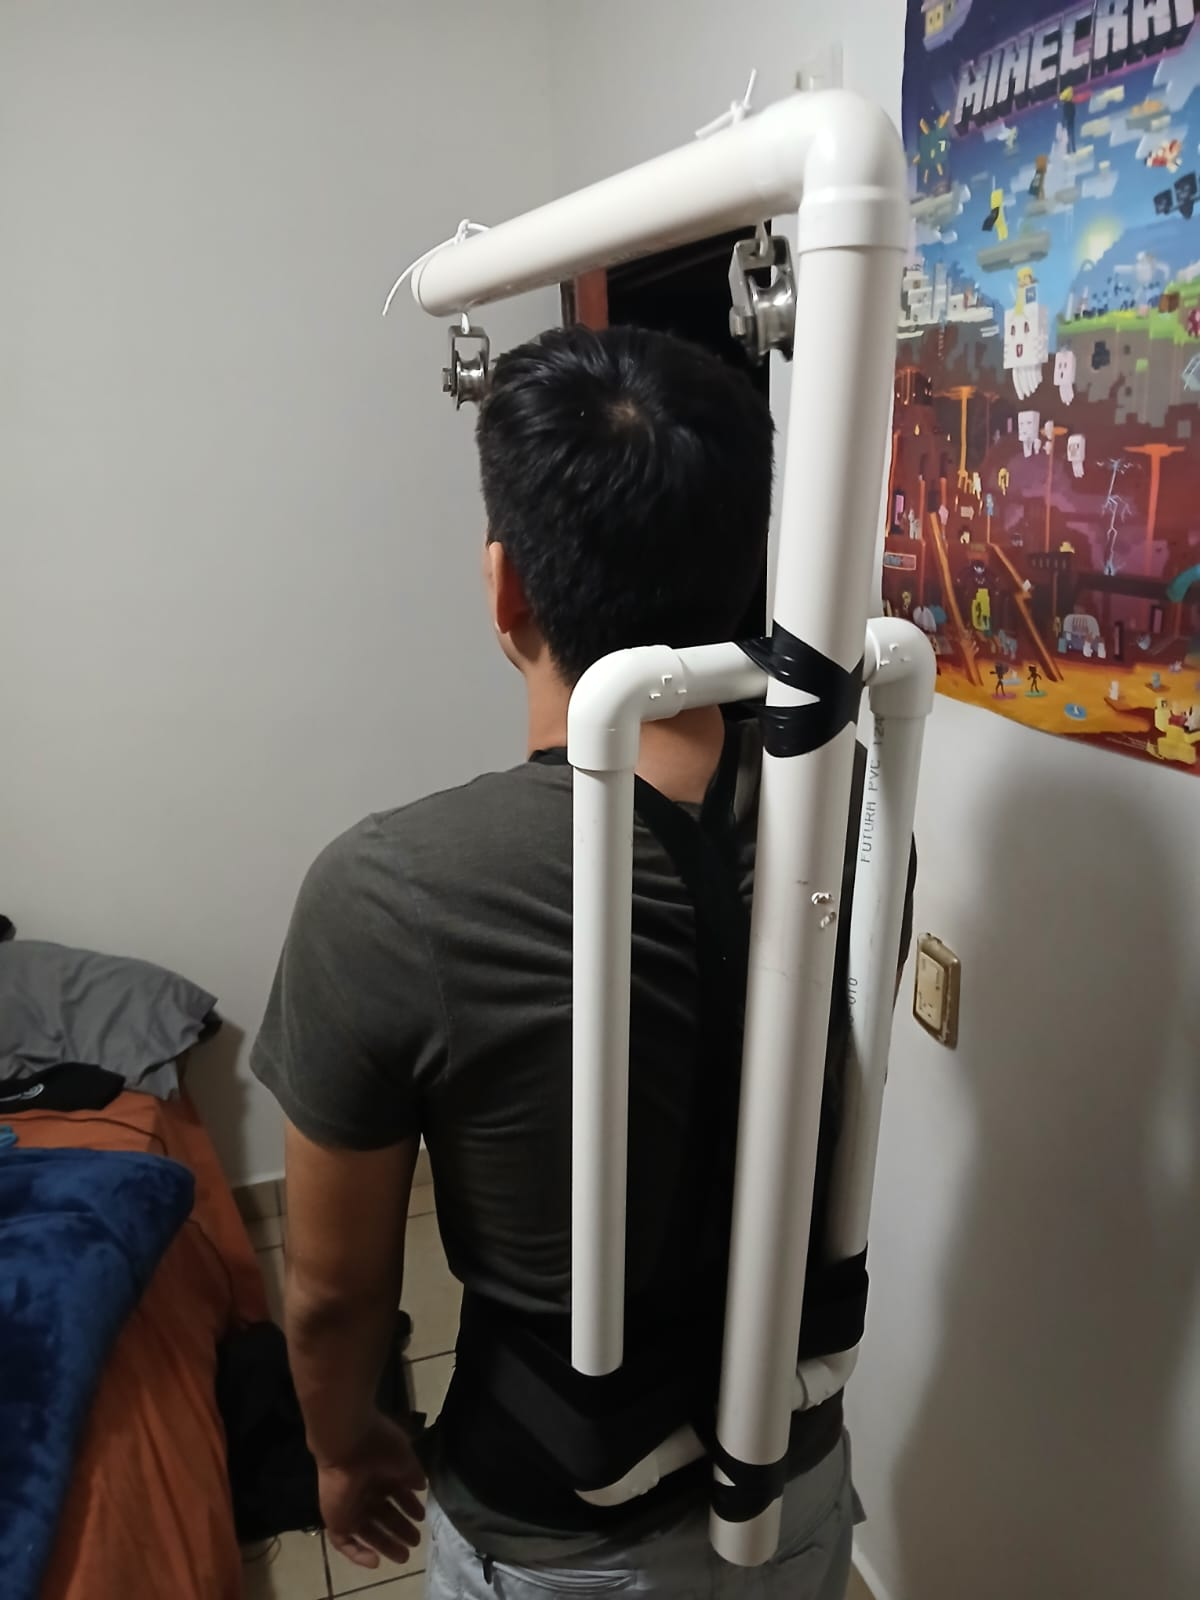
\includegraphics[width=1\textwidth, height=.9\textheight]{img/PruebaErgonomica4.png}
    \caption{Resultados de pruebas de ergonomía}
    \label{fig:ergo-test4}
\end{figure}

\begin{figure}
    \centering
    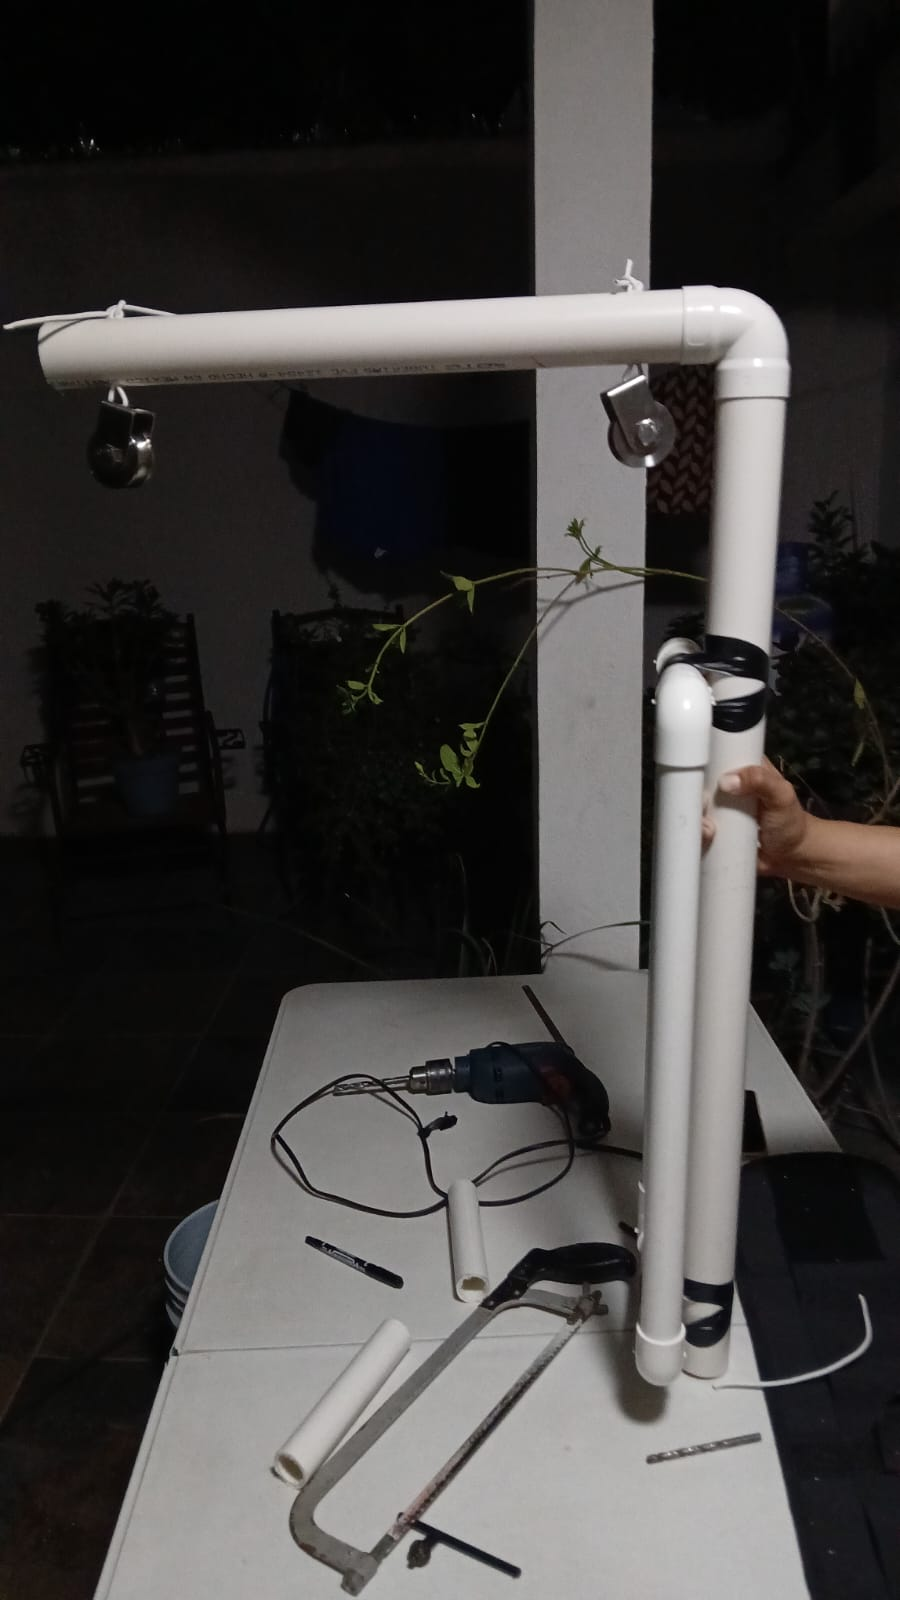
\includegraphics[width=1\textwidth, height=.9\textheight]{img/PruebaErgonomica5.png}
    \caption{Resultados de pruebas de ergonomía}
    \label{fig:ergo-test5}
\end{figure}

\begin{figure}
    \centering
    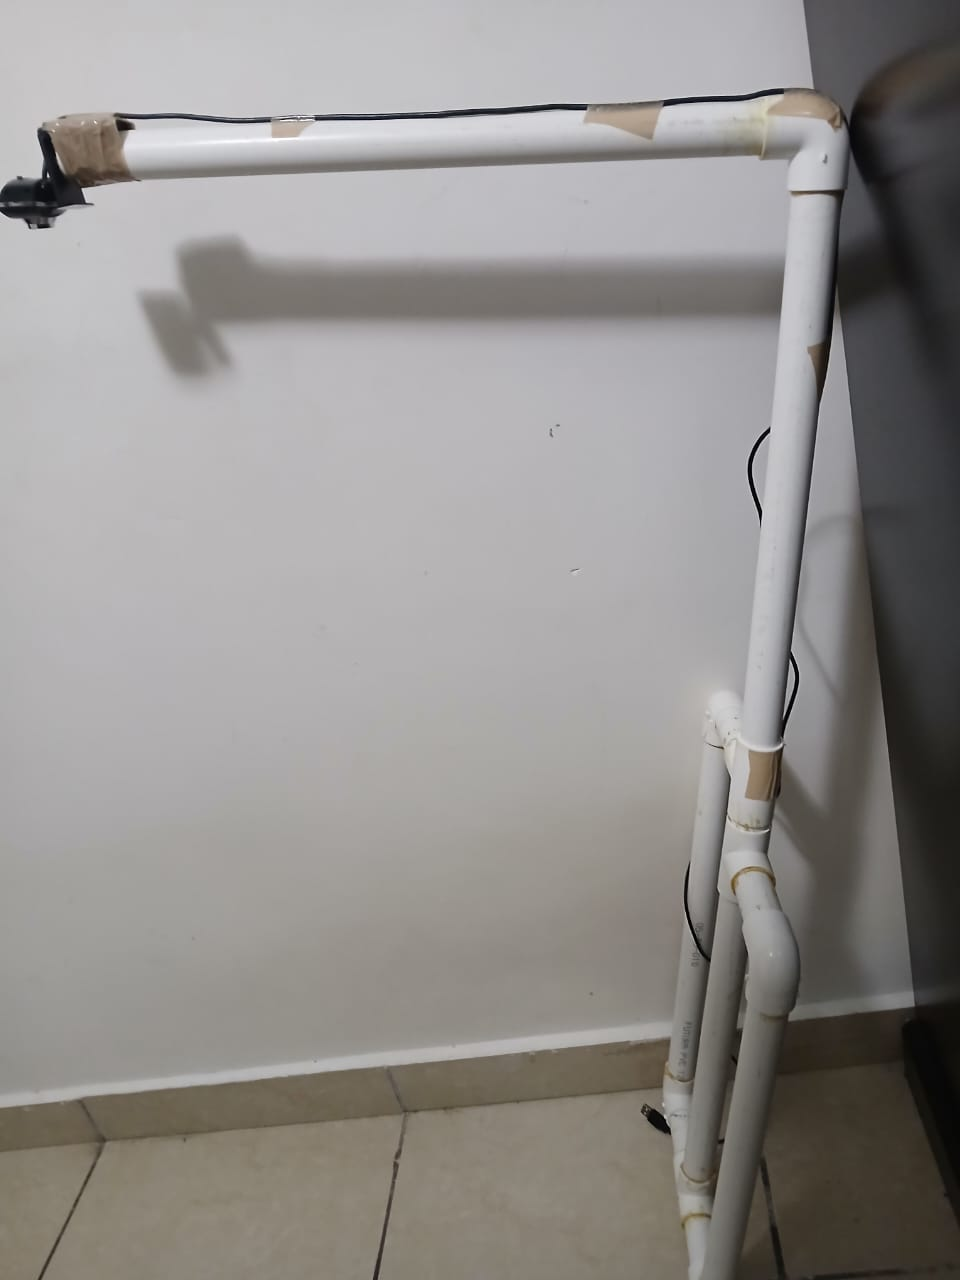
\includegraphics[width=1\textwidth, height=.9\textheight]{img/PruebaErgonomica6.png}
    \caption{Resultados de pruebas de ergonomía}
    \label{fig:ergo-test6}
\end{figure}


\section{Códigos de programación}
Código correspondiente a la Raspberry Pi, donde usando Python con OpenCV y MediaPipe Hands se controla el motor del exoesqueleto:
\begin{minted}[frame=lines, fontsize=\small, linenos, breaklines]{python}
import cv2
import mediapipe as mp
import serial

# Configuración del puerto serial
# arduino = serial.Serial('/dev/ttyUSB0', 9600, timeout=1)  # Ajusta el puerto si es necesario

# Inicializa MediaPipe Hands
mp_hands = mp.solutions.hands
mp_drawing = mp.solutions.drawing_utils
hands = mp_hands.Hands(static_image_mode=False,
                       max_num_hands=2,
                       min_detection_confidence=0.5,
                       min_tracking_confidence=0.5)

def is_hand_open(landmarks):
    """
    Determina si la mano está abierta o cerrada basándose en los puntos clave.
    """
    tip_ids = [4, 8, 12, 16, 20]
    open_fingers = 0

    # Pulgar
    if landmarks[tip_ids[0]].x < landmarks[tip_ids[0] - 1].x:  # Mano derecha
        open_fingers += 1

    # Otros dedos
    for tip_id in tip_ids[1:]:
        if landmarks[tip_id].y < landmarks[tip_id - 2].y:  # Yema más arriba que la articulación
            open_fingers += 1

    return open_fingers >= 4  # Mano abierta si al menos 4 dedos están extendidos

# Captura de video
cap = cv2.VideoCapture('/dev/video0', cv2.CAP_V4L2)

if not cap.isOpened():
    print("No se pudo abrir la cámara.")
    exit()

# Estado inicial
previous_hand_detected = False  # Estado anterior inicial (ninguna mano detectada)
stable_iterations_required = 5  # Iteraciones consecutivas necesarias para confirmar un cambio
current_stable_iterations = 0  # Contador de iteraciones consecutivas estables
current_state = False  # Estado actual confirmado

while True:
    ret, frame = cap.read()
    if not ret:
        print("No se pudo capturar el frame.")
        break

    # Convierte a RGB para MediaPipe
    rgb_frame = cv2.cvtColor(frame, cv2.COLOR_BGR2RGB)

    # Procesa la imagen para detectar manos
    result = hands.process(rgb_frame)

    # Determina si se detectan manos en el cuadro actual
    current_hand_detected = result.multi_hand_landmarks is not None

    # Incrementa o reinicia el contador según el estado detectado
    if current_hand_detected == previous_hand_detected:
        current_stable_iterations += 1
    else:
        current_stable_iterations = 0
        previous_hand_detected = current_hand_detected

    # Verifica si el estado ha sido estable durante las iteraciones necesarias
    if current_stable_iterations >= stable_iterations_required and current_hand_detected != current_state:
        current_state = current_hand_detected
        if current_hand_detected:
            print("Se detecta una mano - Soltar el motor")
            # arduino.write(b'RELEASE\n')  # Enviar comando para soltar el motor
        else:
            print("No se detecta ninguna mano - Retraer el motor")
            # arduino.write(b'RETRACT\n')  # Enviar comando para retraer el motor

    # Dibuja las manos detectadas en el marco
    if result.multi_hand_landmarks:
        for hand_landmarks in result.multi_hand_landmarks:
            mp_drawing.draw_landmarks(frame, hand_landmarks, mp_hands.HAND_CONNECTIONS)

    # Muestra el video con los resultados
    cv2.imshow("Video en tiempo real", frame)

    # Presiona 'q' para salir
    if cv2.waitKey(1) & 0xFF == ord('q'):
        break

cap.release()
cv2.destroyAllWindows()
\end{minted}

Código correspondiente al Arduino, donde se controla el motor del exoesqueleto recibiendo por el puerto serial los comandos enviados desde la Raspberry Pi:
% c code with a caption
\begin{minted}[frame=lines, fontsize=\small, linenos, breaklines]{c}
// Declarar los pines en el Arduino
const int PinIN1 = 5; // Pin digital 5
const int PinIN2 = 4; // Pin digital 4

void setup() {
  // Inicializar la comunicación serial a 9600 baudios
  Serial.begin(9600);

  // Configuramos los pines como salida
  pinMode(PinIN1, OUTPUT);
  pinMode(PinIN2, OUTPUT);

  // Apagar el motor al inicio
  digitalWrite(PinIN1, LOW);
  digitalWrite(PinIN2, LOW);
}

void loop() {
  // Verificar si hay datos disponibles en el puerto serial
  if (Serial.available() > 0) {
    // Leer el comando enviado desde la Raspberry Pi
    String command = Serial.readStringUntil('\n'); // Leer hasta un salto de línea
    command.trim(); // Eliminar espacios o caracteres innecesarios

    // Verificar el comando recibido y ejecutar la acción correspondiente
    if (command == "1") {
      MotorHorario();
      Serial.println("Motor retraído (girando en sentido horario)");
    } else if (command == "2") {
      MotorAntihorario();
      Serial.println("Motor soltando (girando en sentido antihorario)");
    } else if (command == "0" || command == "-1") {
      PararMotor();
      Serial.println("Motor detenido");
    }
  }
}

// Función para girar el motor en sentido horario (retraer)
void MotorHorario() {
  digitalWrite(PinIN1, HIGH);
  digitalWrite(PinIN2, LOW);
}

// Función para girar el motor en sentido antihorario (soltar)
void MotorAntihorario() {
  digitalWrite(PinIN1, LOW);
  digitalWrite(PinIN2, HIGH);
}

// Función para detener el motor
void PararMotor() {
  digitalWrite(PinIN1, LOW);
  digitalWrite(PinIN2, LOW);
}
\end{minted}

\section{Resultados de pruebas de inteligencia artificial}
\begin{figure}[H]
    \centering
    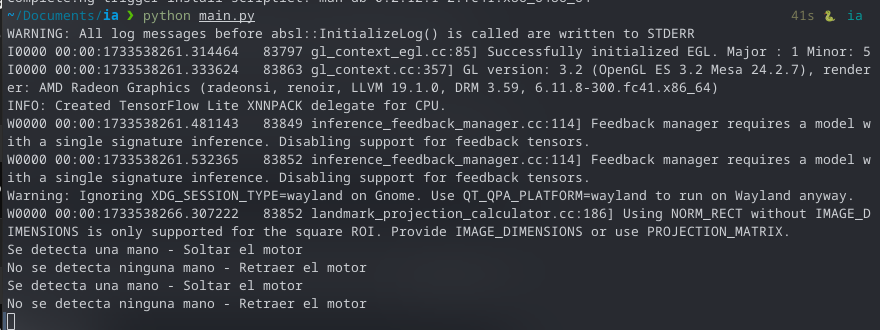
\includegraphics[width=1\textwidth]{img/PruebaIA1.png}
    \caption{Resultados de pruebas de inteligencia artificial}
    \label{fig:ai-test1}
\end{figure}

\begin{figure}[H]
    \centering
    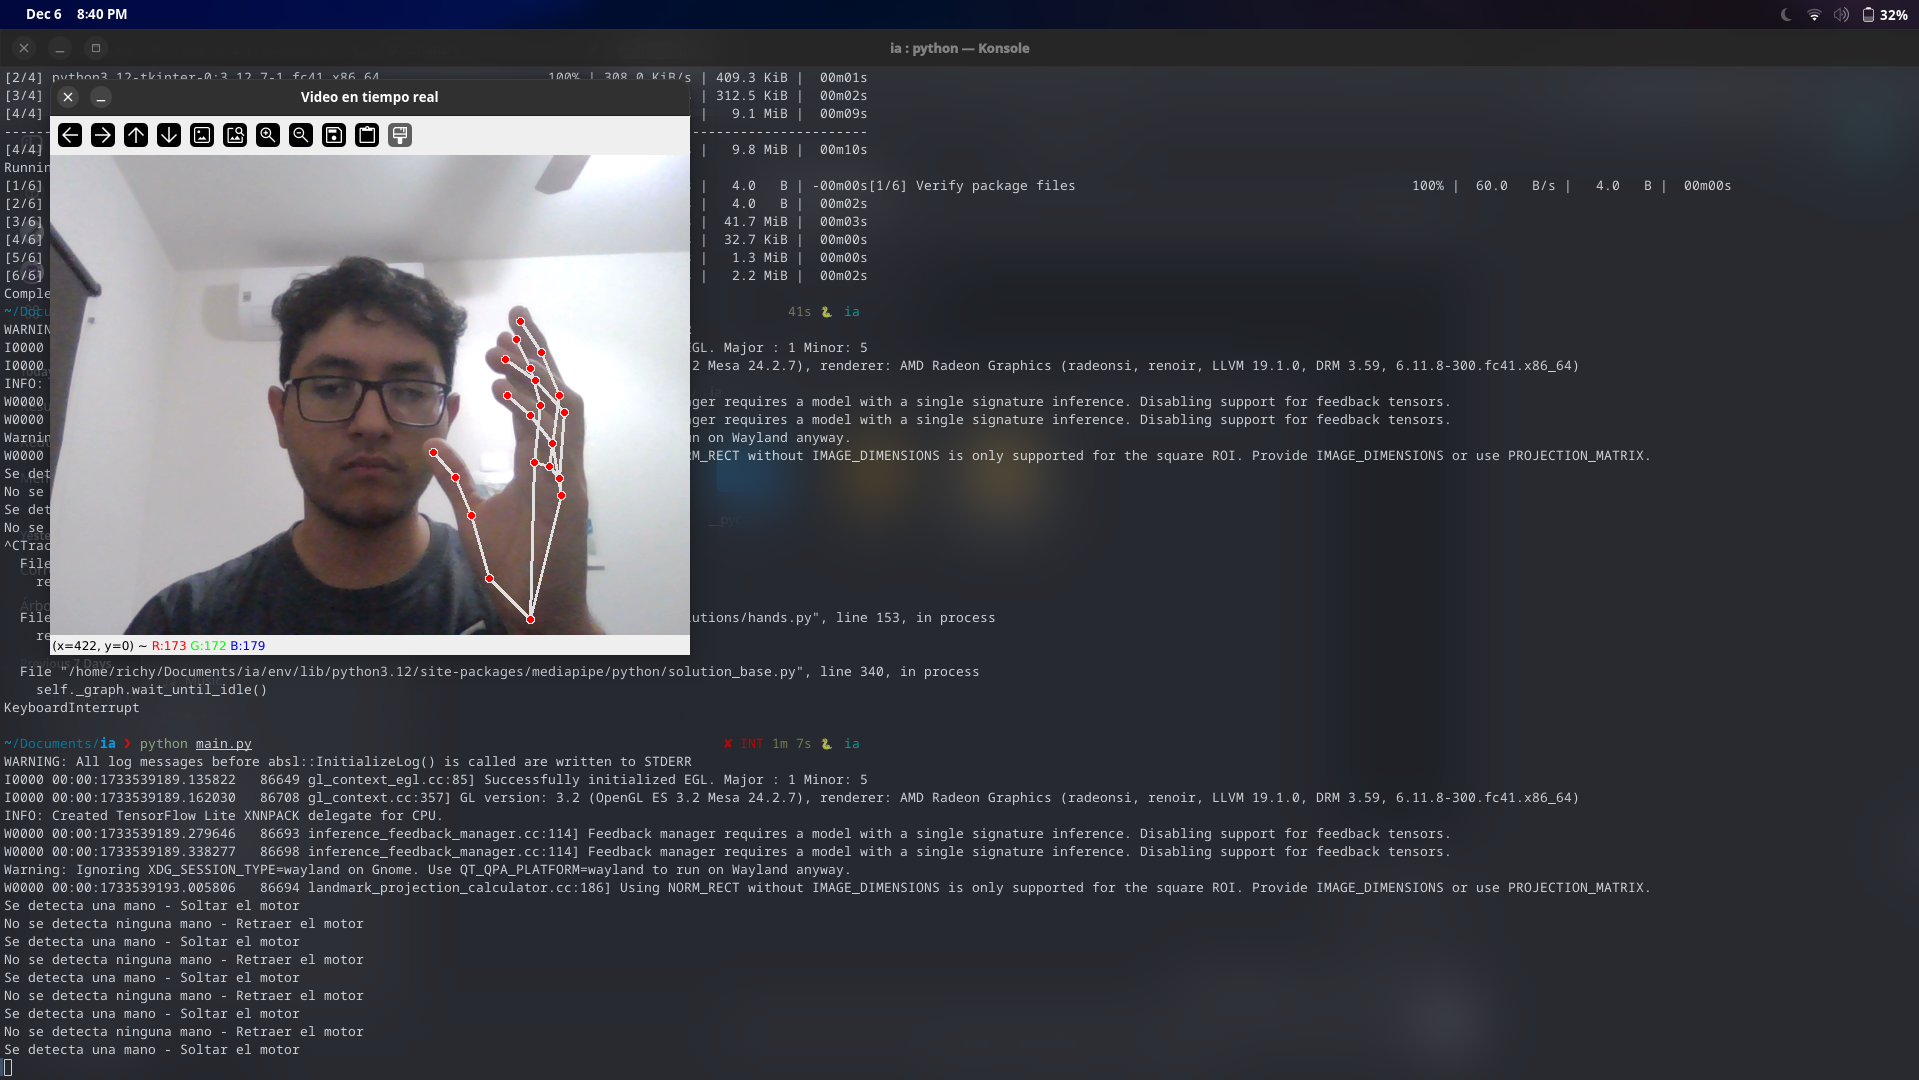
\includegraphics[width=1\textwidth]{img/PruebaIA2.png}
    \caption{Resultados de pruebas de inteligencia artificial}
    \label{fig:ai-test2}
\end{figure}

\begin{figure}[H]
    \centering
    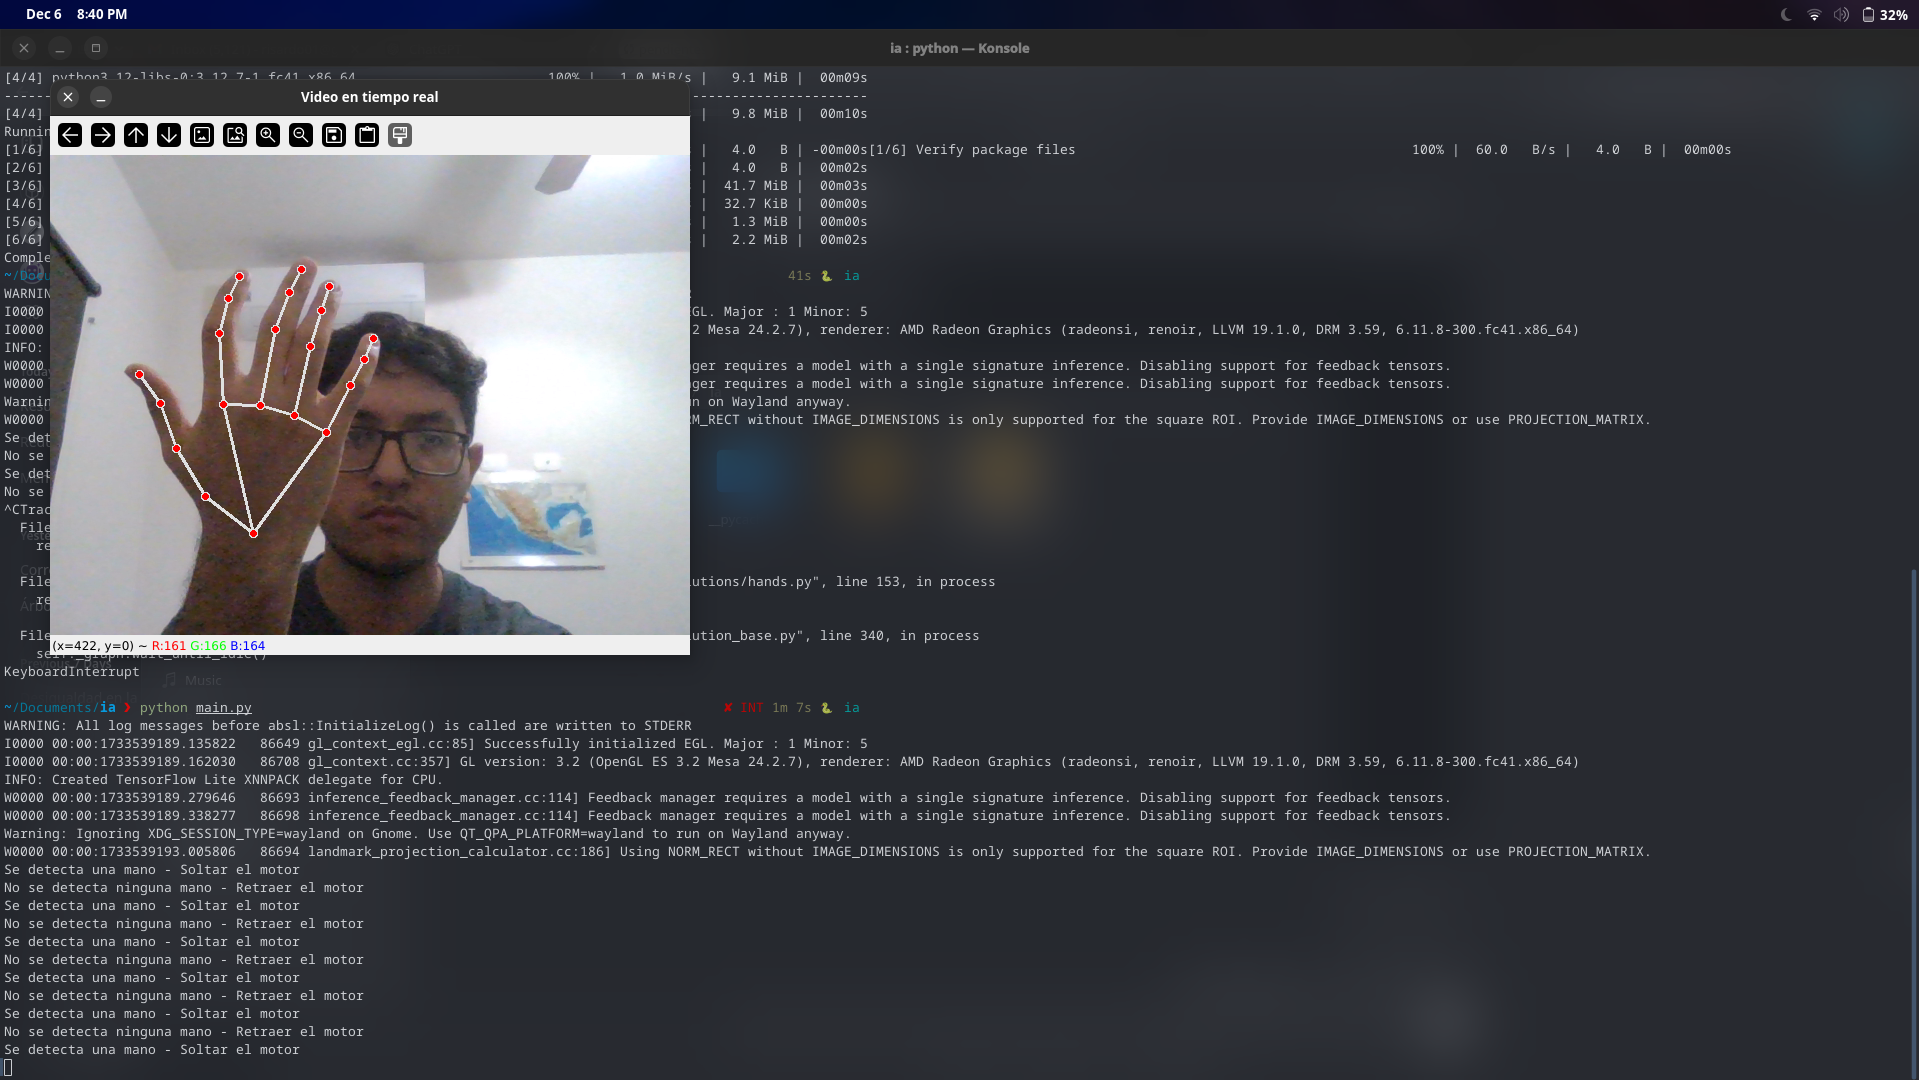
\includegraphics[width=1\textwidth]{img/PruebaIA3.png}
    \caption{Resultados de pruebas de inteligencia artificial}
    \label{fig:ai-test3}
\end{figure}

\begin{figure}[H]
    \centering
    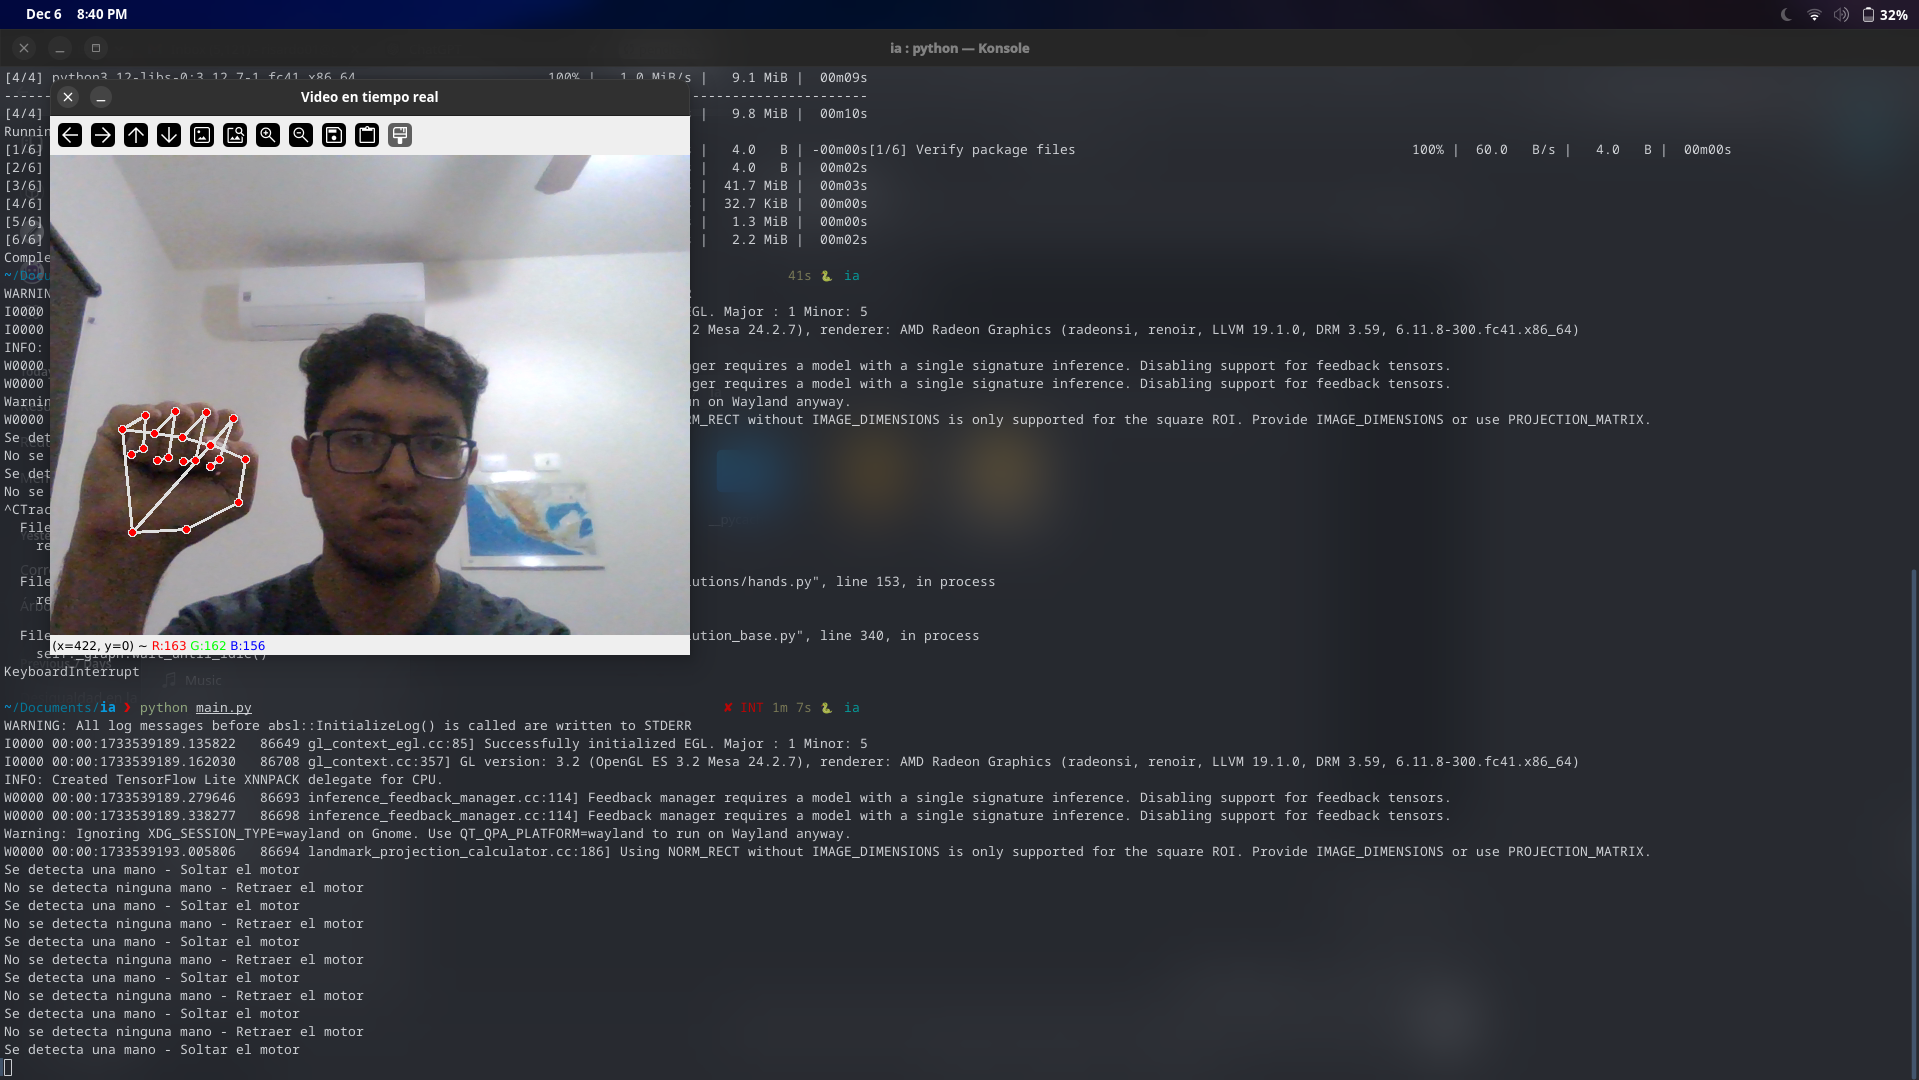
\includegraphics[width=1\textwidth]{img/PruebaIA4.png}
    \caption{Resultados de pruebas de inteligencia artificial}
    \label{fig:ai-test4}
\end{figure}

\begin{figure}[H]
    \centering
    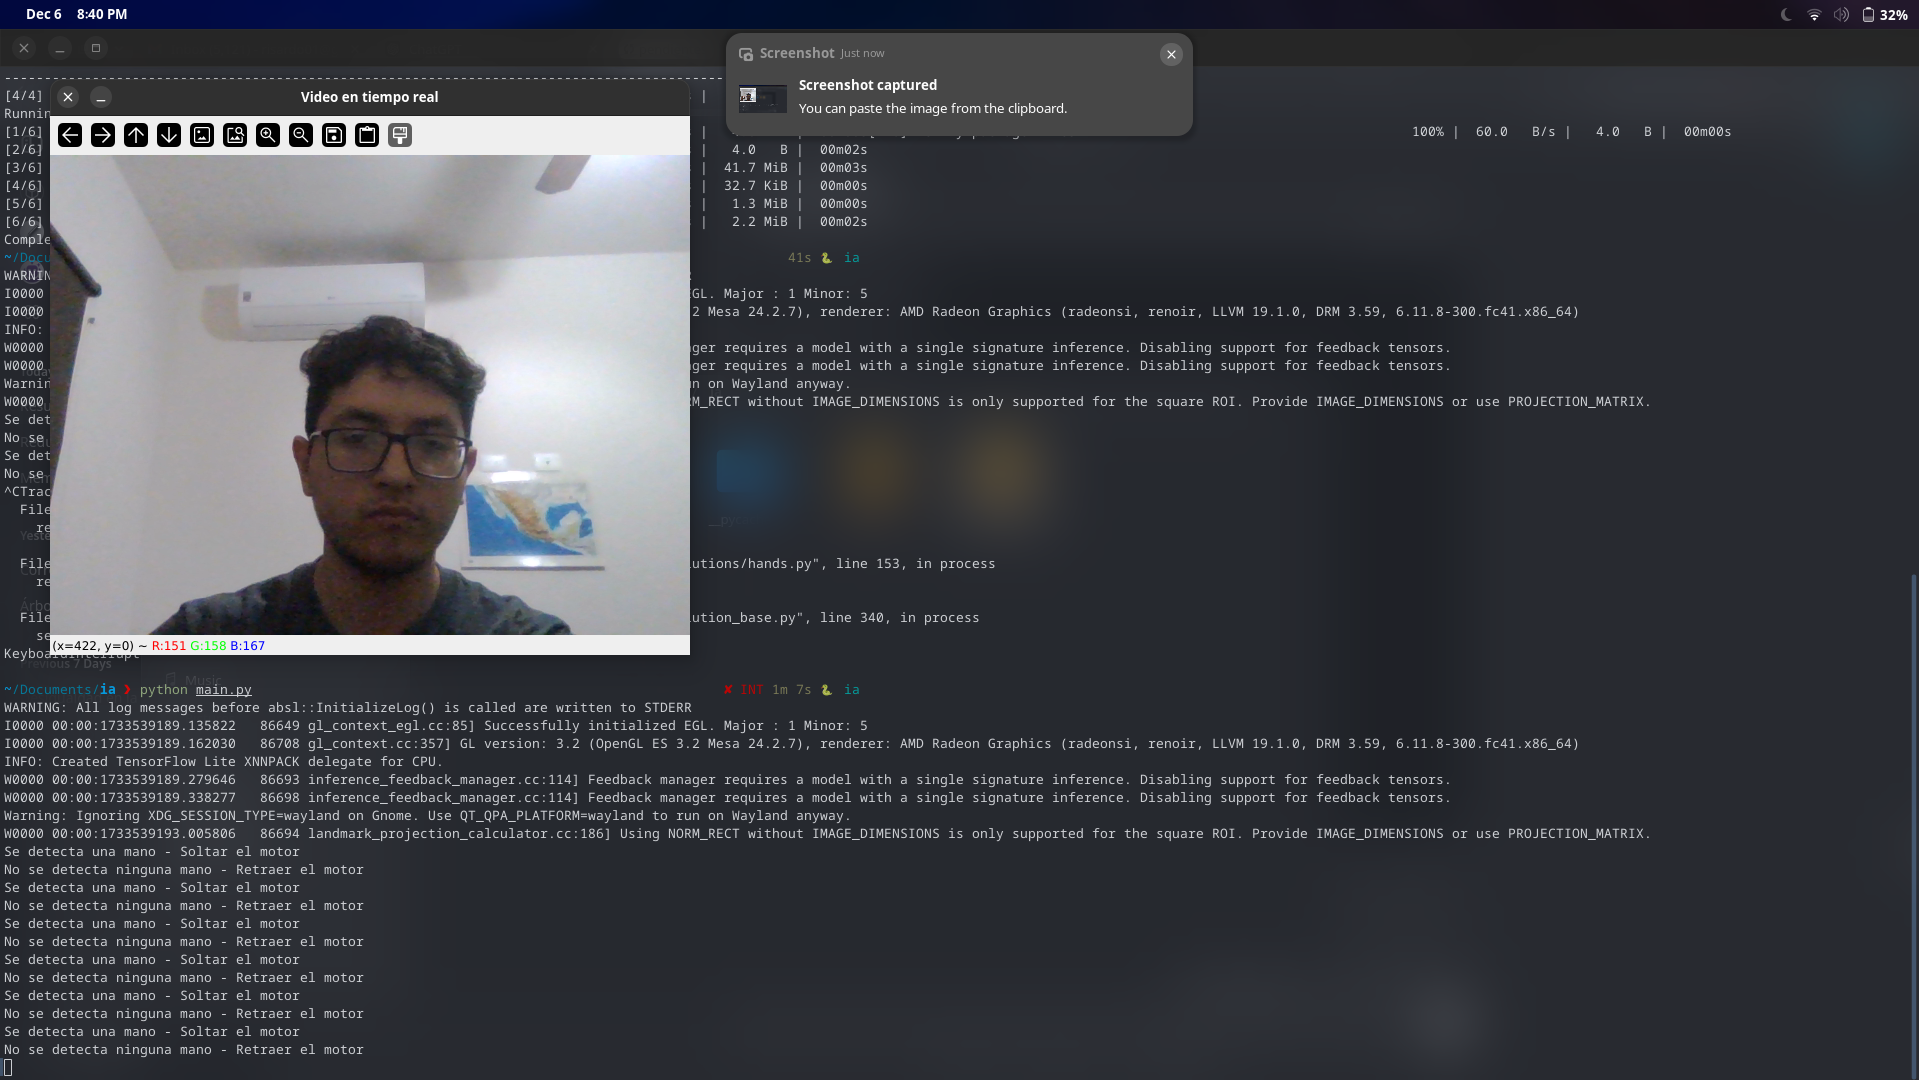
\includegraphics[width=1\textwidth]{img/PruebaIA5.png}
    \caption{Resultados de pruebas de inteligencia artificial}
    \label{fig:ai-test5}
\end{figure}

\begin{figure}[H]
    \centering
    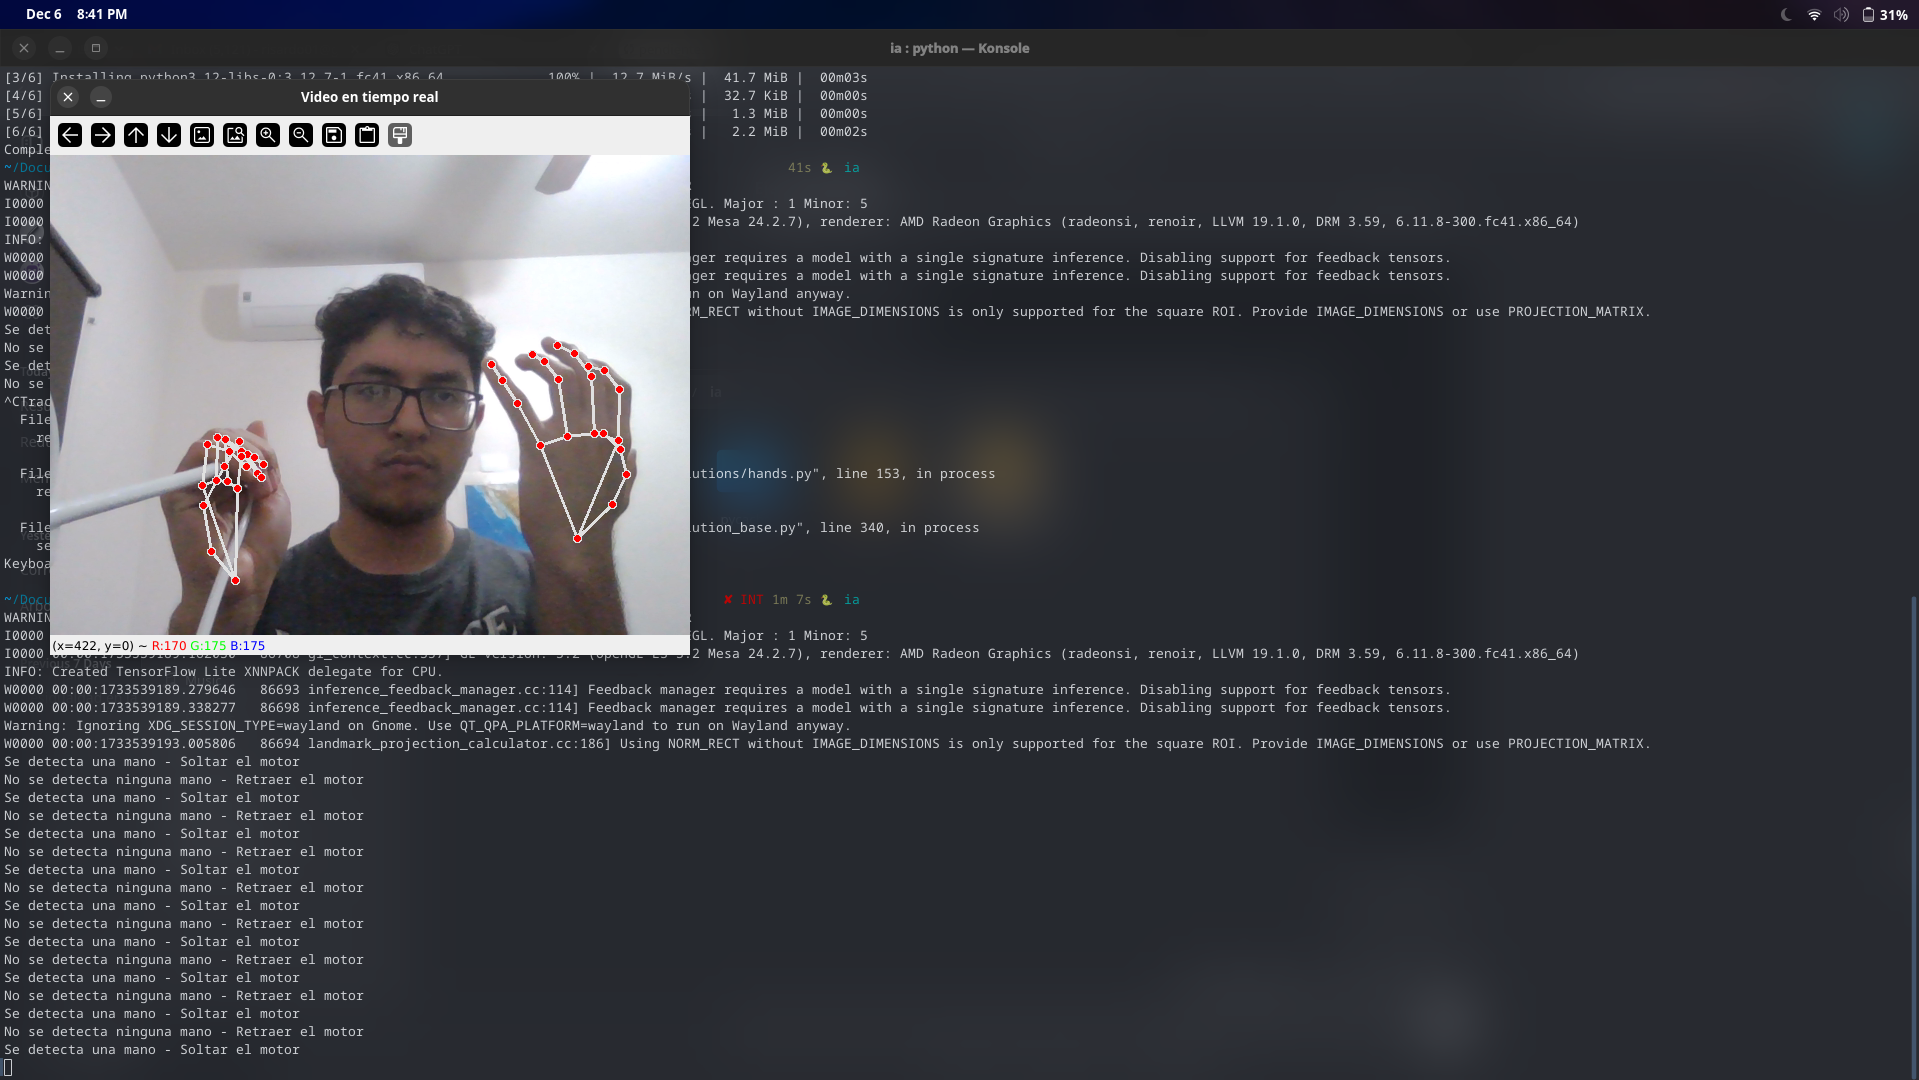
\includegraphics[width=1\textwidth]{img/PruebaIA6.png}
    \caption{Resultados de pruebas de inteligencia artificial}
    \label{fig:ai-test6}
\end{figure}

\begin{figure}[H]
    \centering
    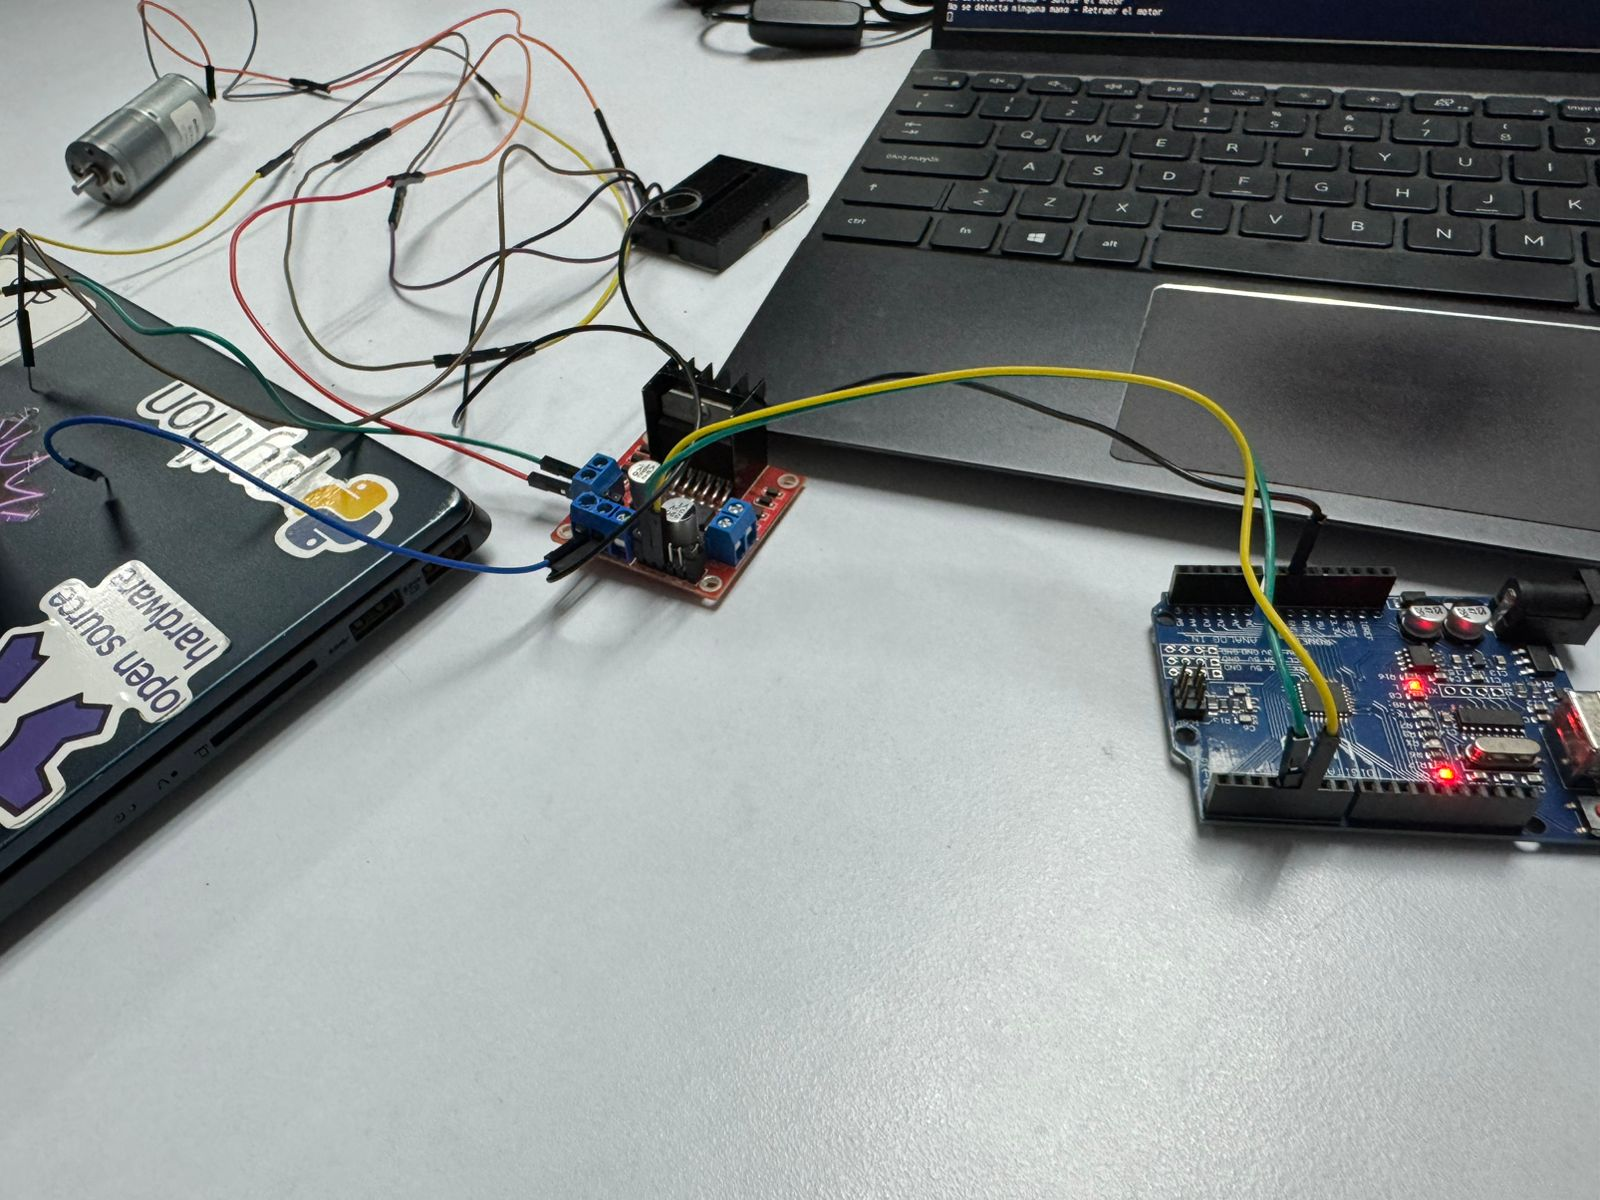
\includegraphics[width=1\textwidth]{img/PruebaIA7.png}
    \caption{Resultados de pruebas de inteligencia artificial}
    \label{fig:ai-test7}
\end{figure}

\begin{figure}[H]
    \centering
    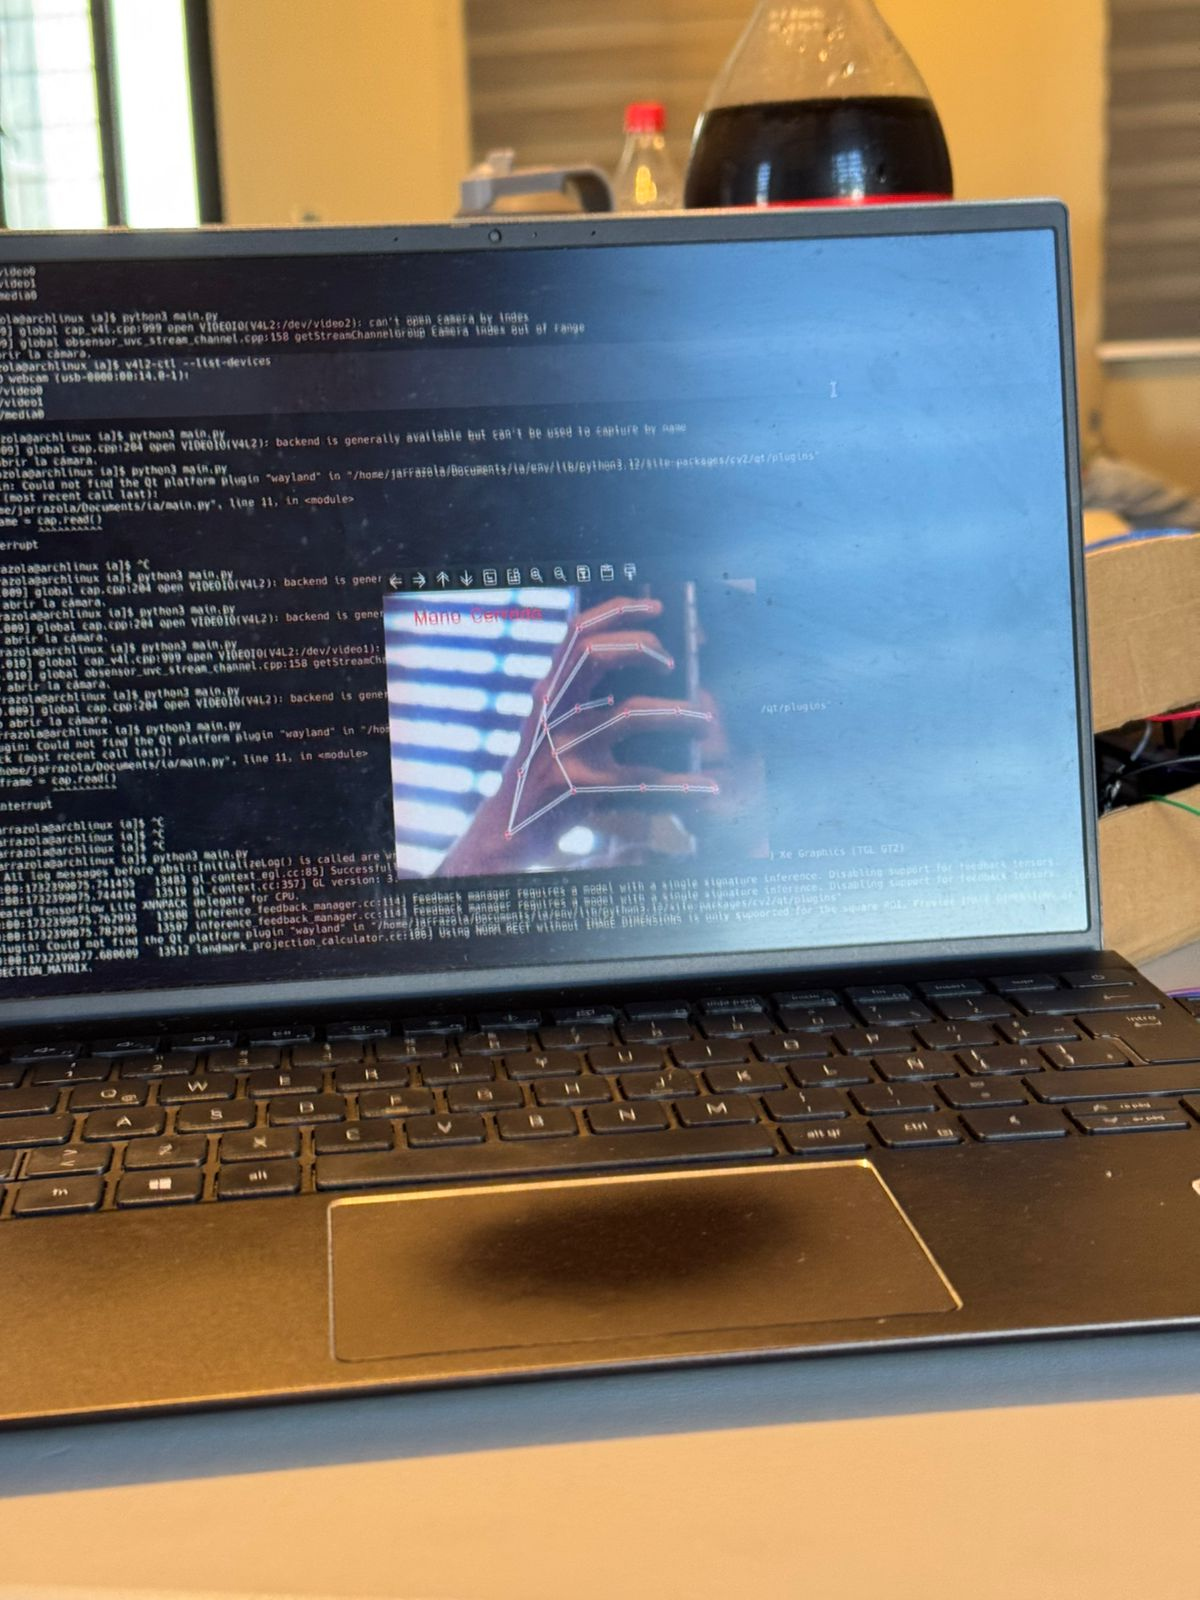
\includegraphics[width=1\textwidth]{img/PruebaIA8.png}
    \caption{Resultados de pruebas de inteligencia artificial}
    \label{fig:ai-test8}
\end{figure}

\begin{figure}[H]
    \centering
    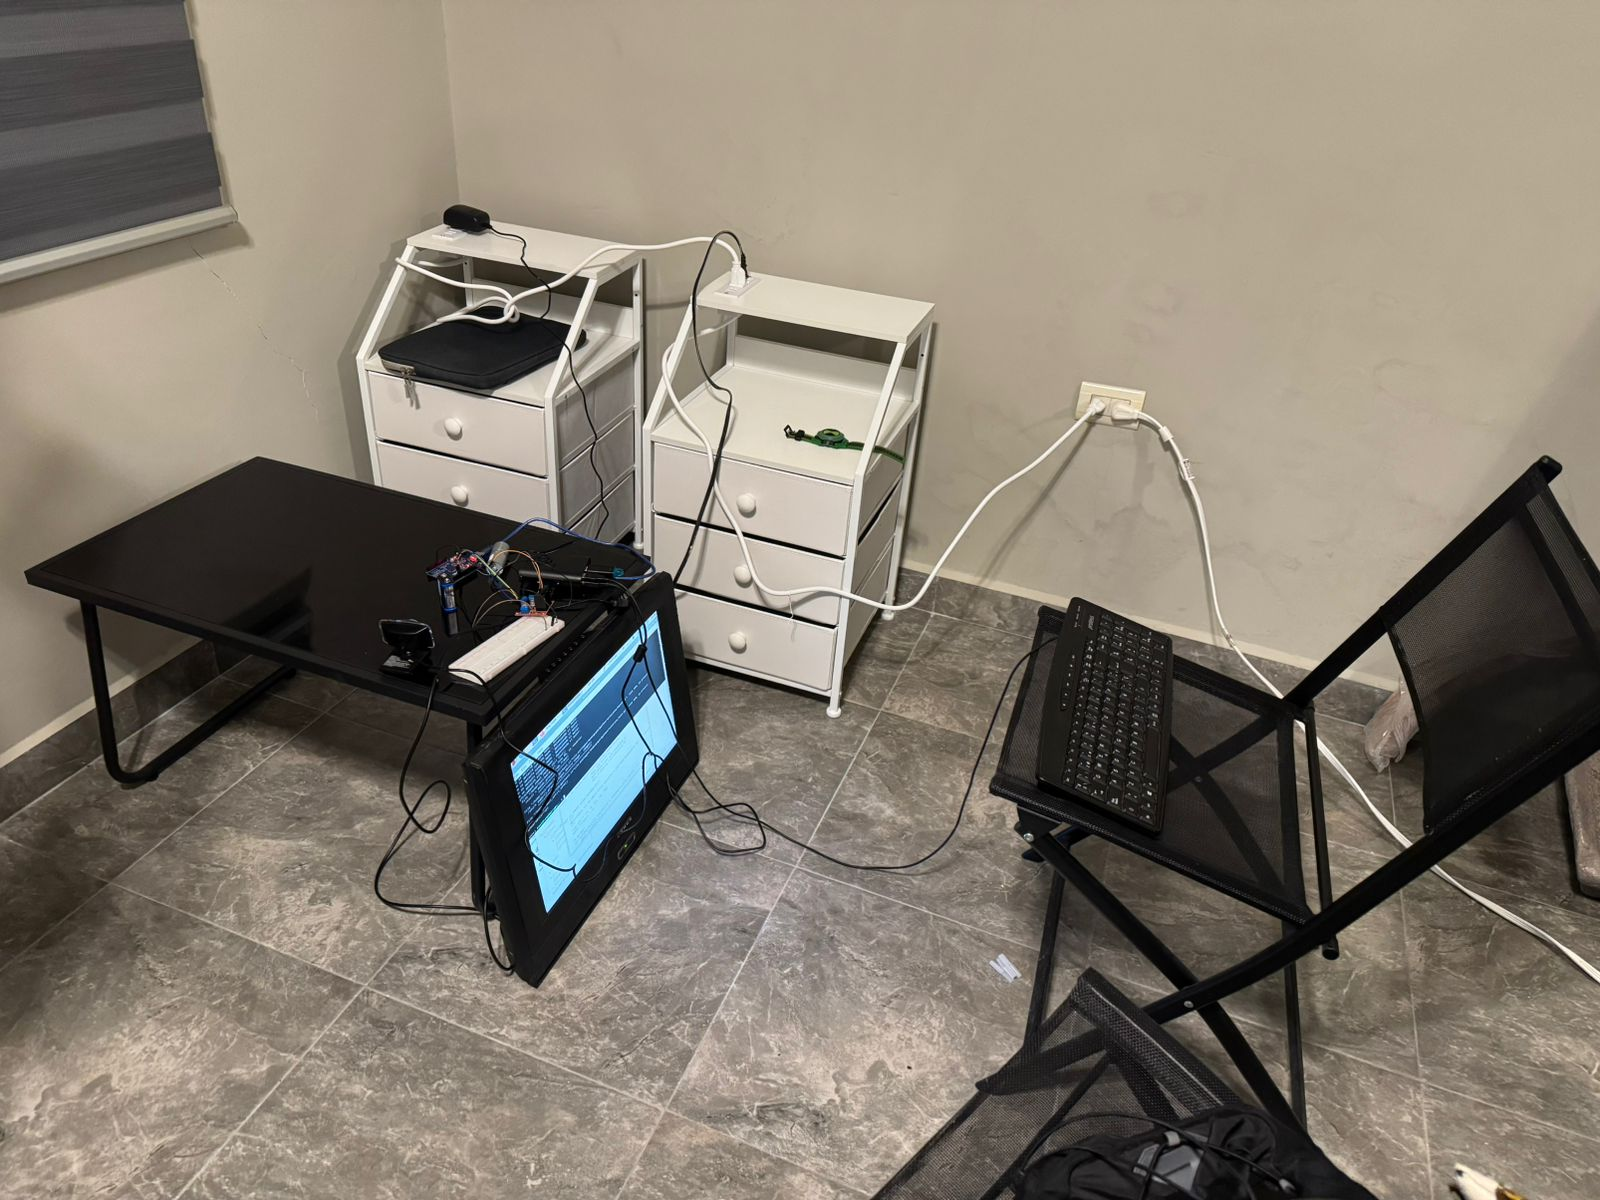
\includegraphics[width=1\textwidth]{img/PruebaIA9.png}
    \caption{Resultados de pruebas de inteligencia artificial}
    \label{fig:ai-test9}
\end{figure}


% \section{Evidencias}